%%
%% This is file `sample-sigconf.tex',
%% generated with the docstrip utility.
%%
%% The original source files were:
%%
%% samples.dtx  (with options: `sigconf')
%% 
%% IMPORTANT NOTICE:
%% 
%% For the copyright see the source file.
%% 
%% Any modified versions of this file must be renamed
%% with new filenames distinct from sample-sigconf.tex.
%% 
%% For distribution of the original source see the terms
%% for copying and modification in the file samples.dtx.
%% 
%% This generated file may be distributed as long as the
%% original source files, as listed above, are part of the
%% same distribution. (The sources need not necessarily be
%% in the same archive or directory.)
%%
%%
%% Commands for TeXCount
%TC:macro \cite [option:text,text]
%TC:macro \citep [option:text,text]
%TC:macro \citet [option:text,text]
%TC:envir table 0 1
%TC:envir table* 0 1
%TC:envir tabular [ignore] word
%TC:envir displaymath 0 word
%TC:envir math 0 word
%TC:envir comment 0 0
%%
%%
%% The first command in your LaTeX source must be the \documentclass command.

%\documentclass[sigconf]{acmart}
%\documentclass[sigconf,screen]{acmart}

\documentclass[sigconf,review,anonymous]{acmart}
\acmConference[ESEC/FSE 2023]{The 31st ACM Joint European Software Engineering Conference and Symposium on the Foundations of Software Engineering}{11 - 17 November, 2023}{San Francisco, USA}

%%
%% \BibTeX command to typeset BibTeX logo in the docs
\AtBeginDocument{%
  \providecommand\BibTeX{{%
    Bib\TeX}}}

\usepackage{booktabs}   %% For formal tables:
                        %% http://ctan.org/pkg/booktabs
\usepackage{subcaption} %% For complex figures with subfigures/subcaptions
                        %% http://ctan.org/pkg/subcaption
\usepackage{array}
\usepackage{amsmath,amsfonts}
\usepackage{algorithm}
\usepackage[noend]{algpseudocode}
%\usepackage{algorithmic}
\usepackage{graphicx}
\usepackage{textcomp}
\usepackage{float}
\usepackage{listings}
\usepackage{xspace}
\usepackage{multirow}
\usepackage{amsthm}
\newtheorem{definition}{Definition}
\usepackage{balance}

\usepackage[skins]{tcolorbox}

\usepackage{xcolor,pifont}
\newcommand*\colourcheck[1]{%
	\expandafter\newcommand\csname #1check\endcsname{\textcolor{#1}{\ding{52}}}%
}
\colourcheck{blue}
\colourcheck{green}
\colourcheck{red}

\newtcolorbox{myframe}[2][]{%
  enhanced,colback=white,colframe=black,coltitle=black,
  sharp corners,
  toprule=1.0pt,
  rightrule=0.3pt,
  leftrule=0pt,
  bottomrule=0pt,
  fonttitle=\itshape\scshape\large,
  left=0pt,right=5pt,top=5pt,bottom=3pt,
  attach boxed title to top right={yshift=-0.3\baselineskip-0.4pt,xshift=-5mm},
  boxed title style={tile,size=minimal,left=0.2mm,right=0.5mm,
    colback=white,before upper=\strut},
  title=#2,#1
}

\newcommand{\tool}{\textsc{DeepFQN}\xspace}

%\newcommand{\mvpdg}{$\delta$-PDG$^{i,j}$}

\newtheorem{Definition}{Definition}
\newtheorem{Claim}{Claim}
\newtheorem{Lemma}{Lemma}
\newtheorem{Theorem}{Theorem}

\newcolumntype{L}[1]{>{\raggedright\arraybackslash}p{#1}}
\newtheorem{observation}{Observation}
\newtheorem{property}{Property}
\newcommand{\code}[1]{{\footnotesize\texttt{#1}}}
\usepackage{amsthm}
 \definecolor{dkgreen}{rgb}{0,0.6,0}
\definecolor{gray}{rgb}{0.5,0.5,0.5}
\definecolor{mauve}{rgb}{0.58,0,0.82}
\lstset{frame=tb,
  language=Java,
  aboveskip=3mm,
  belowskip=3mm,
  showstringspaces=false,
  columns=flexible,
  basicstyle={\small\ttfamily},
  numbers=left,
  numberstyle=\tiny\color{gray},
  keywordstyle=\color{blue},
  commentstyle=\color{dkgreen},
  stringstyle=\color{mauve},
  breaklines=true,
  breakatwhitespace=true,
  tabsize=4
}

%% Rights management information.  This information is sent to you
%% when you complete the rights form.  These commands have SAMPLE
%% values in them; it is your responsibility as an author to replace
%% the commands and values with those provided to you when you
%% complete the rights form.
%\setcopyright{acmcopyright}
%\copyrightyear{2018}
%\acmYear{2018}
%\acmDOI{XXXXXXX.XXXXXXX}

%% These commands are for a PROCEEDINGS abstract or paper.
%\acmConference[Conference acronym 'XX]{Make sure to enter the correct
%  conference title from your rights confirmation emai}{June 03--05,
%  2018}{Woodstock, NY}
%\acmPrice{15.00}
%\acmISBN{978-1-4503-XXXX-X/18/06}


%%% If you see 'ACMUNKNOWN' in the 'setcopyright' statement below,
%%% please first submit your publishing-rights agreement with ACM (follow link on submission page).
%%% Then please update our instructions page and copy-and-paste the NEW commands into your article.
%%% Please contact us in case of questions; allow up to 10 min for the system to propagate the information.
%%%

%%% The following is specific to ESEC/FSE '22 and the paper
%%% 'UTANGO: Untangling Commits with Context-Aware, Graph-Based, Code Change Clustering Learning Model'
%%% by Yi Li, Shaohua Wang, and Tien N. Nguyen.
%%%

%\setcopyright{acmcopyright}
%\acmPrice{15.00}
%\acmDOI{10.1145/3540250.3549171}
%\acmYear{2022}
%\copyrightyear{2022}
%\acmSubmissionID{fse22main-p1469-p}
%\acmISBN{978-1-4503-9413-0/22/11}
%\acmConference[ESEC/FSE '22]{Proceedings of the 30th ACM Joint European Software Engineering Conference and Symposium on the Foundations of Software Engineering}{November 14--18, 2022}{Singapore, Singapore}
%\acmBooktitle{Proceedings of the 30th ACM Joint European Software Engineering Conference and Symposium on the Foundations of Software Engineering (ESEC/FSE '22), November 14--18, 2022, Singapore, Singapore}

%\setcopyright{ACMUNKNOWN}
%\acmPrice{15.00}
%\acmDOI{10.1145/3540250.3549137}
%\acmYear{2022}
%\copyrightyear{2022}
%\acmSubmissionID{fse22main-p639-p}
%\acmISBN{978-1-4503-9413-0/22/11}
%\acmConference[ESEC/FSE '22]{Proceedings of the 30th ACM Joint European Software Engineering Conference and Symposium on the Foundations of Software Engineering}{November 14--18, 2022}{Singapore, Singapore}
%\acmBooktitle{Proceedings of the 30th ACM Joint European Software Engineering Conference and Symposium on the Foundations of Software Engineering (ESEC/FSE '22), November 14--18, 2022, Singapore, Singapore}

%\copyrightyear{2022}
%\acmYear{2022}
%\setcopyright{acmcopyright}
%\acmConference[ESEC/FSE '22]{Proceedings of the 30th ACM Joint European Software Engineering Conference and Symposium on the Foundations of Software Engineering}{November 14--18, 2022}{Singapore, Singapore}
%\acmBooktitle{Proceedings of the 30th ACM Joint European Software Engineering Conference and Symposium on the Foundations of Software Engineering (ESEC/FSE '22), November 14--18, 2022, Singapore, Singapore}
%\acmPrice{15.00}
%\acmDOI{10.1145/3540250.3549137}
%\acmISBN{978-1-4503-9413-0/22/11}


%%
%% Submission ID.
%% Use this when submitting an article to a sponsored event. You'll
%% receive a unique submission ID from the organizers
%% of the event, and this ID should be used as the parameter to this command.
%%\acmSubmissionID{123-A56-BU3}

%%
%% For managing citations, it is recommended to use bibliography
%% files in BibTeX format.
%%
%% You can then either use BibTeX with the ACM-Reference-Format style,
%% or BibLaTeX with the acmnumeric or acmauthoryear sytles, that include
%% support for advanced citation of software artefact from the
%% biblatex-software package, also separately available on CTAN.
%%
%% Look at the sample-*-biblatex.tex files for templates showcasing
%% the biblatex styles.
%%

%%
%% The majority of ACM publications use numbered citations and
%% references.  The command \citestyle{authoryear} switches to the
%% "author year" style.
%%
%% If you are preparing content for an event
%% sponsored by ACM SIGGRAPH, you must use the "author year" style of
%% citations and references.
%% Uncommenting
%% the next command will enable that style.
%%\citestyle{acmauthoryear}



%%
%% end of the preamble, start of the body of the document source.
\begin{document}

%%
%% The "title" command has an optional parameter,
%% allowing the author to define a "short title" to be used in page headers.
%\title{The Name of the Title Is Hope}

\title[Title goes here]{Title goes here}

\setcopyright{none}

\settopmatter{printacmref=false, printfolios=false}

\renewcommand\footnotetextcopyrightpermission[1]{} % removes footnote with conference information in first column

%%
%% The "author" command and its associated commands are used to define
%% the authors and their affiliations.
%% Of note is the shared affiliation of the first two authors, and the
%% "authornote" and "authornotemark" commands
%% used to denote shared contribution to the research.

%\author{Ben Trovato}
%\authornote{Both authors contributed equally to this research.}
%\email{trovato@corporation.com}
%\orcid{1234-5678-9012}
%\author{G.K.M. Tobin}
%\authornotemark[1]
%\email{webmaster@marysville-ohio.com}
%\affiliation{%
%  \institution{Institute for Clarity in Documentation}
%  \streetaddress{P.O. Box 1212}
%  \city{Dublin}
%  \state{Ohio}
%  \country{USA}
%  \postcode{43017-6221}
%}

%\author{Lars Th{\o}rv{\"a}ld}
%\affiliation{%
%  \institution{The Th{\o}rv{\"a}ld Group}
%  \streetaddress{1 Th{\o}rv{\"a}ld Circle}
%  \city{Hekla}
%  \country{Iceland}}
%\email{larst@affiliation.org}

%\author{Valerie B\'eranger}
%\affiliation{%
%  \institution{Inria Paris-Rocquencourt}
%  \city{Rocquencourt}
%  \country{France}
%}

%\author{Aparna Patel}
%\affiliation{%
% \institution{Rajiv Gandhi University}
% \streetaddress{Rono-Hills}
% \city{Doimukh}
% \state{Arunachal Pradesh}
% \country{India}}

%\author{Huifen Chan}
%\affiliation{%
%  \institution{Tsinghua University}
%  \streetaddress{30 Shuangqing Rd}
%  \city{Haidian Qu}
%  \state{Beijing Shi}
%  \country{China}}

%\author{Charles Palmer}
%\affiliation{%
%  \institution{Palmer Research Laboratories}
%  \streetaddress{8600 Datapoint Drive}
%  \city{San Antonio}
%  \state{Texas}
%  \country{USA}
%  \postcode{78229}}
%\email{cpalmer@prl.com}

%\author{John Smith}
%\affiliation{%
%  \institution{The Th{\o}rv{\"a}ld Group}
%  \streetaddress{1 Th{\o}rv{\"a}ld Circle}
%  \city{Hekla}
%  \country{Iceland}}
%\email{jsmith@affiliation.org}

%\author{Julius P. Kumquat}
%\affiliation{%
%  \institution{The Kumquat Consortium}
%  \city{New York}
%  \country{USA}}
%\email{jpkumquat@consortium.net}

%\author{Yi Li}
%\affiliation{
%	\institution{New Jersey Institute of Technology}
%	\state{New Jersey}
%	\country{USA}
%}
%\email{yl622@njit.edu}
%\author{Shaohua Wang}
%\authornote{Corresponding Author}
%\affiliation{
%	\institution{New Jersey Institute of Technology}
%	\state{New Jersey}
%	\country{USA}
%}
%\email{davidsw@njit.edu}
%\author{Tien N. Nguyen}
%\affiliation{
%	\institution{University of Texas at Dallas}
%	\state{Texas}
%	\country{USA}
%}
%\email{tien.n.nguyen@utdallas.edu}

%\renewcommand{\shortauthors}{Yi Li, Shaohua Wang, and Tien N. Nguyen}


%%
%% By default, the full list of authors will be used in the page
%% headers. Often, this list is too long, and will overlap
%% other information printed in the page headers. This command allows
%% the author to define a more concise list
%% of authors' names for this purpose.

%\renewcommand{\shortauthors}{Trovato et al.}

%%
%% The abstract is a short summary of the work to be presented in the
%% article.

\begin{abstract}
Abstract goes here.
\end{abstract}

%Our empirical evaluation on a C\# dataset with 1,612 tangled commits
%shows that it achieves the accuracy of 28.6\%--462.5\%, relatively
%higher than the state-of-the-art approaches in clustering the changed
%code. We evaluated {\tool} in a Java dataset with +14k
%tangled commits. The result shows that it achieves 13.3\%--100.0\%
%relatively higher accuracy than the state-of-the-art~approaches.



%Exploring this duality provides useful constraints for {\tool} to
%learn derive CC fixing statements.

%DEAR and CURE in which we replaced their FL modules with our tool.
%exploit this duality. In a cross-stitch unit, the sharing of
%representations between \code{MethFL} and \code{StmtFL} is modeled by
%the learning a linear combination of the input features from two
%models.  The cross-stitch units

%%
%% The code below is generated by the tool at http://dl.acm.org/ccs.cfm.
%% Please copy and paste the code instead of the example below.
%%

%% Keywords. The author(s) should pick words that accurately describe
%% the work being presented. Separate the keywords with commas.
%\keywords{Commit Untangling; Deep Learning; Code Change Embeddings}

%% A "teaser" image appears between the author and affiliation
%% information and the body of the document, and typically spans the
%% page.
%\begin{teaserfigure}
%  \includegraphics[width=\textwidth]{sampleteaser}
%  \caption{Seattle Mariners at Spring Training, 2010.}
%  \Description{Enjoying the baseball game from the third-base
%  seats. Ichiro Suzuki preparing to bat.}
%  \label{fig:teaser}
%\end{teaserfigure}

%%
%% This command processes the author and affiliation and title
%% information and builds the first part of the formatted document.

\maketitle

\section{Introduction}
\label{sec:intro}

Software libraries and frameworks play important roles in software
development. Their functionality is provided via the Application
Programming Interface (API) elements including classes, methods, and
fields. The online forums, e.g., StackOverflow or GitHub Gists, have
provided an excellent resource on how to use API
elements. Unfortunately, due to the current context of the discussions
in such forums, the code snippets in the answering StackOverflow posts
may contain the ambiguities on the references to the API elements of
the external libraries~\cite{liveapi14}.

Several approaches have been proposed to automatically resolve the
fully qualified names (FQNs) of the API elements for the code snippets
in the public forums.  The approaches can be classified into different
categories. The first category is {\em program analysis}. Partial
program analysis~\cite{dagenais-oopsla08} derives the types and FQNs
in a best-effort manner. RecoDoc~\cite{dagenais-icse12} utilizes
several heuristics on syntactic constructs to recognize the names.
The second category is {\em information
  retrieval}. Baker~\cite{liveapi14} builds a candidate list for each
name by tracking the scopes of the names and then overlapping the
lists according to the scoping rules to narrow down the candidates.
COSTER~\cite{coster-ase19} captures the context of the query API
element and matches that with the FQNs of API elements with three
criteria on likelihood, context similarity, and name similarity.  The
third category is {\em constraint-based}.  SnR~\cite{snr-icse22}
builds a knowledge base of APIs, i.e., various facts about the
available APIs.  SnR extracts typing constraints from the given
snippet, and solves the constraints against the knowledge base. The
fourth category leverages the advances in {\em artificial intelligence
  (AI) and machine learning (ML)}. StatType considers the problem of
deriving FQNs as the machine translation from the code without FQNs to
the one with them. Huang {\em et al.}~\cite{prompt-ase22} formulate
the problem as a fill-in-blank task using a masked language model. The
approach fills in the FQN for each name considering the context
consisting of the few lines before and after the fill-in location.
The key issue is that the API elements are designed to use in
different client code, making the surrounding contexts different for
different code using the APIs.

Instead of characterizing the surrounding context
of the fill-in location (i.e., the location of an API element),
we ...


\section{Motivation}
\label{motiv:sec}

\subsection{Motivating Examples}
\label{examples:sec}

%https://stackoverflow.com/questions/4531396/get-value-of-a-edit-text-field/4531500#4531500: SO post #4531500
\begin{figure}[htbp]
	\centering
	\lstset{
		numbers=left,
		numberstyle= \tiny,
		keywordstyle= \color{blue!70},
		commentstyle= \color{red!50!green!50!blue!50},
		frame=shadowbox,
		rulesepcolor= \color{red!20!green!20!blue!20} ,
		xleftmargin=1.5em,xrightmargin=0em, aboveskip=1em,
		framexleftmargin=1.5em,
                numbersep= 5pt,
		language=C,
    basicstyle=\scriptsize\ttfamily,
    numberstyle=\scriptsize\ttfamily,
    emphstyle=\bfseries,
                moredelim=**[is][\color{red}]{@}{@},
		escapeinside= {(*@}{@*)}
	}
\begin{lstlisting}[]
(*@{\color{blue}{Button}@*)   mButton;
EditText mEdit;

(*@@@*)Override public (*@{\color{black}{void}@*) onCreate(Bundle savedInstanceState) {
    super.onCreate(savedInstanceState);
    setContentView(R.layout.main);

    (*@{\color{blue}mButton = findViewById(R.id.button);@*)
    mEdit   = (EditText)findViewById(R.id.edittext);

    (*@{\color{blue}mButton.setOnClickListener(@*)
        (*@{\color{purple}new View.OnClickListener()@*)
        {
            public (*@{\color{black}{void}@*) onClick(View view)
            {
                Log.v("EditText", mEdit.getText().toString());
            }
        });
}
\end{lstlisting}
        \vspace{-12pt}
        \caption{StackOverflow Post \#4531500 on Android Library}
        \label{fig:example1}
\end{figure}


Let us examine some real-world examples to help motivate our approach. Fig.~\ref{fig:example1} illustrates a code snippet of an answer to S/O question \#4531500 on the Android library. Due to the informal discourse in S/O, code snippets rarely contain the necessary declarations and references to the fully-qualified names (FQNs); and often lack the import statements. Besides, the references to external types are also unqualified since the responder assumes that those FQNs can be implicitly understood from the context of the post. For example, in Fig.~\ref{fig:example1}, the types \code{Button} (line 1), \code{EditText} (line 2), \code{Bundle} (line 4), \code{View} (line 14), or \code{Log} (line 16) are referenced only by their simple names. Thus, the code will not be compilable unless the corresponding import statements are added.

%https://stackoverflow.com/questions/18323473/how-to-implement-gwt-java-button-and-the-clickhandler
\begin{figure}[htbp]
	\centering
	\lstset{
		numbers=left,
		numberstyle= \tiny,
		keywordstyle= \color{blue!70},
		commentstyle= \color{red!50!green!50!blue!50},
		frame=shadowbox,
		rulesepcolor= \color{red!20!green!20!blue!20} ,
		xleftmargin=1.5em,xrightmargin=0em, aboveskip=1em,
		framexleftmargin=1.5em,
                numbersep= 5pt,
		language=C,
    basicstyle=\scriptsize\ttfamily,
    numberstyle=\scriptsize\ttfamily,
    emphstyle=\bfseries,
                moredelim=**[is][\color{red}]{@}{@},
		escapeinside= {(*@}{@*)}
	}
\begin{lstlisting}[]
public class myClass implements EntryPoint {
    final (*@{\color{blue}{Button}@*) myButton = new (*@{\color{blue}{Button}@*)("text");
    (*@{\color{blue}{myButton.addClickHandler(}@*)
        (*@{\color{purple}{new ClickHandler() \{}@*)
            public (*@{\color{black}{void}@*) onClick(ClickEvent event) {
               onClickMyButton(event);
        }
    });
    private (*@{\color{black}{void}@*) onClickMyButton(ClickEvent event) {
            ... 
    }
}
\end{lstlisting}
        \vspace{-12pt}
        \caption{StackOverflow Post \#18323473 on GWT Library}
        \label{fig:example2}
\end{figure}


Moreover, the APIs of external libraries are prone to name ambiguity, meaning that they can be confused with other APIs from different libraries that share the same name and offer a similar functionality. For example, the element \code{Button} on line 1 in Fig.~\ref{fig:example1} is a common unqualified type. Here, it refers to \code{android.widget.Button}. Next, consider Fig.~\ref{fig:example2}, which illustrates a code snippet of an answer to a S/O post on Google Web Toolkit (GWT). Because this code snippet does not contain any import statements and the references to the APIs are also unqualified, the type \code{Button} on line 2 in Fig.~\ref{fig:example2} is ambiguous from that on line 1 in Fig.~\ref{fig:example1}. Such name ambiguity in type names is a common phenomenon, especially among S/O code snippets. For instance, the simple name \code{getId} occurs 27,434 times across various Java libraries~\cite{liveapi14}.

\subsection{Observations}
\label{sec:obs}

We can observe a need for a tool that automatically derives the fully-qualified names of the API elements in code snippets from online forums. This will facilitate the reuse of such incomplete code by enabling the addition of the appropriate import statements. To build one such tool, we draw motivation from the following observations.

\vspace{2pt}
\noindent {\bf Observation 1} [{\em Regularity of API Usages}]. The designers of software libraries intend for developers to use the API elements together (including API classes, method calls, and field accesses) in certain combinations/orders to achieve a task. For example, in the GWT code snippet illustrated in Fig.~\ref{fig:example2}, a variable of the type \code{Button} (FQN: \code{com.google.gwt.user.client.ui.Button}) is instantiated on line 2. Then, on line 3, to set the handler of that GWT button, one needs to invoke the \code{addClickHandler} method (FQN: \code{com.google.gwt.user.client.ui.Button.add\-Click\-Handler})  on the \code{Button} object with an argument of the type \code{ClickHandler} (FQN: \code{com\-.google\-.gwt\-.event\-.dom\-.client\-.ClickHandler}). Thus, they are intended to be used in  such a combination and will appear together frequently.

Next, in Fig.~\ref{fig:example3}, we illustrate a complete code example published on the GWT tutorial website \code{gwtproject.org}. Here, the author provides all necessary \code{import} statements and demonstrates how to use different GUI elements in GWT. Specifically, consider the \code{Button} object declared with the \code{addStockButton} variable name on line 12. It calls the method \code{addClickHandler} on line 23 with an argument of the same type as earlier, \code{ClickHandler}. 
%Though the \code{Button} object is assigned with different variable names in both cases, i.e., \code{myButton} when incomplete, and \code{addStockButton} when complete, we can see that the combination of these API elements can help establish its identity in the form of its FQN. 
Despite being assigned with different variable names in both the complete and incomplete cases, i.e., \code{myButton} and \code{addStockButton} respectively, we can see that the combination of these API elements can help establish \code{Button} object's identity and resolve its FQN.

In brief, the source code in public repositories is a good source for a model to implicitly learn the API usages and derive the FQNs of the API elements in an incomplete snippet.

%https://www.gwtproject.org/doc/latest/tutorial/manageevents
\begin{figure}[htbp]
	\centering
	\lstset{
		numbers=left,
		numberstyle= \tiny,
		keywordstyle= \color{blue!70},
		commentstyle= \color{red!50!green!50!blue!50},
		frame=shadowbox,
		rulesepcolor= \color{red!20!green!20!blue!20} ,
		xleftmargin=1.5em,xrightmargin=0em, aboveskip=1em,
		framexleftmargin=1.5em,
                numbersep= 5pt,
		language=C,
    basicstyle=\scriptsize\ttfamily,
    numberstyle=\scriptsize\ttfamily,
    emphstyle=\bfseries,
                moredelim=**[is][\color{red}]{@}{@},
		escapeinside= {(*@}{@*)}
	}
\begin{lstlisting}[]
import com.google.gwt.core.client.EntryPoint;
import com.google.gwt.event.dom.client.ClickEvent;
import com.google.gwt.event.dom.client.ClickHandler;
import com.google.gwt.user.client.ui.Button;
import com.google.gwt.user.client.ui.HorizontalPanel;
import com.google.gwt.user.client.ui.RootPanel;
import com.google.gwt.user.client.ui.VerticalPanel;
...
public class StockWatcher implements EntryPoint {
  private VerticalPanel mainPanel = new VerticalPanel();
  private HorizontalPanel addPanel = new HorizontalPanel();
  private Button addStockButton = new Button("Add");
  ...
  public void onModuleLoad() {
    ...
    // Assemble Add Stock panel.
    addPanel.add(addStockButton);
    // Assemble Main panel.
    mainPanel.add(addPanel);
    // Associate the Main panel with the HTML host page.
    RootPanel.get("stockList").add(mainPanel);
    // Listen for mouse events on the Add button.
    (*@{\color{blue}{addStockButton.addClickHandler(}@*) (*@{\color{purple}{new ClickHandler() \{}@*)
      public void onClick(ClickEvent event) {
        addStock();
      }
    });
  }
  private void addStock() {
    ...
  }
}
\end{lstlisting}
        \vspace{-12pt}
        \caption{Complete Source Code in gwtproject.org}
        \label{fig:example3}
\end{figure}


\vspace{2pt}
\noindent {\bf Observation 2} [{\em Dependencies/Relations among API Elements in a Usage}].
The API elements used together in an API usage in certain combinations/orders share various program dependencies. These relationships can contribute to identifying the FQNs of the API elements better. For example, in Fig.~\ref{fig:example3}, we can see that to set a handler for a button in GWT, the object of the type \code{Button} needs to be the {\em receiving object of the method call} to \code{addClickHandler}, which in turn needs to accept an object of the type \code{ClickHandler} as an argument. The client code utilizing GWT library for this purpose will demonstrate the relationships shared between these three API elements as well. For example, in Fig.~\ref{fig:example2}, if \code{addClickHandler} on line 3 is determined to be the API element \code{com.\-google.\-gwt.\-user.\-client.\-ui.\-Button.\-add\-Click\-Handler}, the FQN of the element at line 4 must be \code{com\-.google\-.gwt\-.event\-.dom\-.client\-.ClickHandler}. The opposite direction of reasoning is also applicable. In general, if a model can learn the dependencies/relations among API elements in an API usage, it could leverage such knowledge to decide the FQNs of all API elements at the same time.

%the lines 2 and 3 in Fig. 2
As another example, consider the data dependency from the \code{def-use} relationship via the variable \code{myButton} between line~2 and line~3 in Fig.~\ref{fig:example2}. This relationship helps derive the FQNs for the above API elements. For instance, if a model decides the FQN for \code{Button} on line 2 to be \code{com\-.google\-.gwt\-.user\-.client\-.ui\-.Button}, it could consequently derive the FQN of \code{add\-Click\-Handler} on line~3 as \code{com.\-google.\-gwt.\-user.\-client.\-ui.\-Button.\-add\-Click\-Handler}, and vice versa.

\vspace{2pt}
\noindent {\bf State-of-the-Art Approaches.} Several approaches have been proposed to recover the fully-qualified names (FQNs) for the API elements in a code snippet. The {\em program-analysis-based} approaches (e.g., PPA~\cite{dagenais-oopsla08}, RecoDoc~\cite{dagenais-icse12}), {\em information-retrieval-based} approaches (e.g., Baker~\cite{liveapi14}, COSTER~\cite{coster-ase19}), and {\em constraint-based} approaches (e.g., SnR~\cite{snr-icse22}) are not comprehensive, and suffer from out-of-vocabulary failures. %(i.e., cannot derive FQNs that were not seen in the training corpus).

Employing the recent advances in {\em machine} and {\em deep learning} (ML \& DL) for FQN resolution has enabled the generation of new FQNs for API elements. However, the state-of-the-art ML/DL-based approaches (e.g., StatType~\cite{icse18} and Huang {\em et al.}~\cite{prompt-ase22}) {\bf do not yet leverage the regularity in API-usages and the dependencies among the relevant API elements} for FQN prediction. StatType~\cite{icse18} leverages phrase-based statistical machine translation to transform an API type-sequence without FQNs to one with them. However, with only short phrases of lengths between 3-8 tokens, StatType is not capable of capturing long-range dependencies between API elements. For example, in Fig.~\ref{fig:example1}, StatType misses the inter-connections between the statements spanning across 11 lines from \code{Button mButton} on line 1 to \code{mButton}, \code{findViewById}, etc. on line 8; and to \code{mButton}, \code{setOnClickListener} on line 11. Moreover, in some cases, it is possible for two relevant API elements to be even farther in the code snippet.

Huang {\em et al.}~\cite{prompt-ase22} formulated FQN resolution as a fill-in-the-blank problem and leveraged a masked language model (MLM\textsubscript{\textit{FIB}}) for this purpose. They build each training instance by taking the statement at each type inference point (e.g., \code{View} on line 12) and a couple of surrounding lines with unresolved API elements as context. This approach has several limitations. First, the amount of contextual information might not capture all relevant API elements corresponding to the same API-usage. In Fig.~\ref{fig:example1}, \code{mButton} on line 1 is far apart from \code{mButton} on line 8 and \code{mButton} on line 11. Next, individual API elements might be used in a different context in the client code. For example, the code on line 9 in Fig.~\ref{fig:example1} is specific to the method \code{onCreate}. Thus, such limited context might not provide the model with sufficient information for determining the FQN.


%Talk about StatType and fill-in


\section{Important Concepts}
\label{sec:concepts}

This section describes the definitions of the important concepts
regarding our representations on API usages.

\begin{figure}[t] %[!htp]
	\centering
	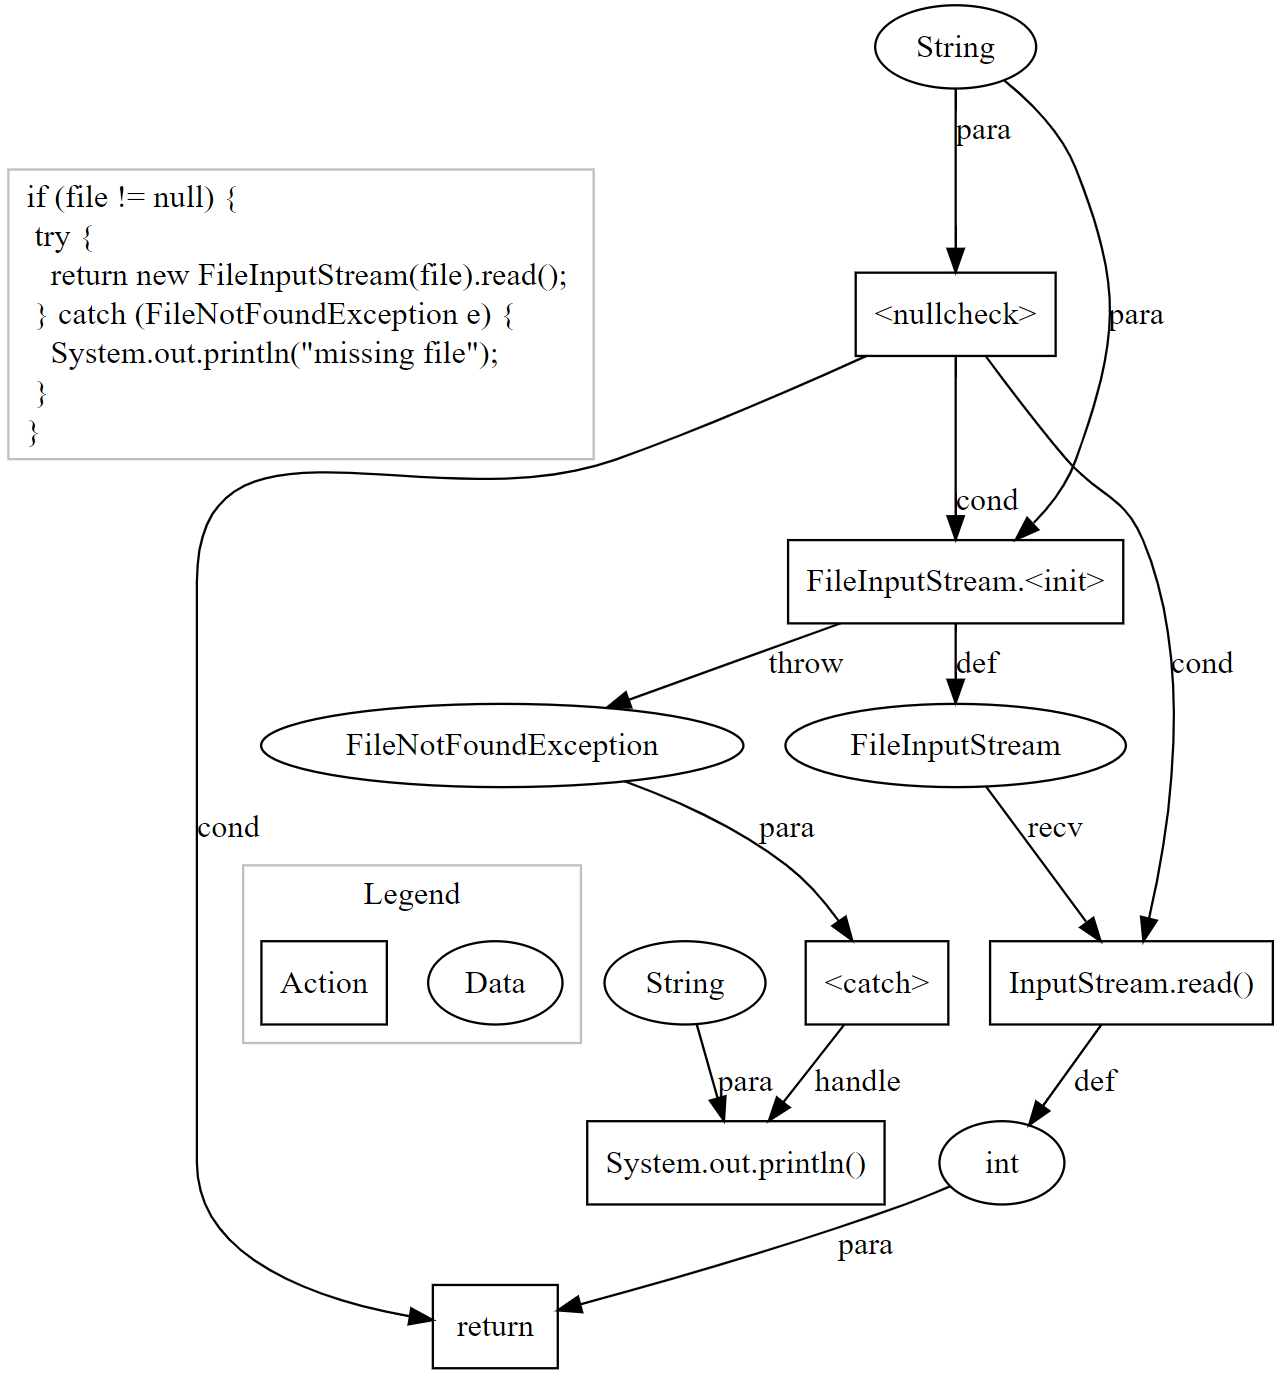
\includegraphics[width=0.9\linewidth]{aug-example}
        \vspace{-3pt}
	\caption{An API Usage and its API-Usage Graph}
	\label{fig:aug}
\end{figure}

\begin{Definition}[API elements]
  An API element is either a class, a method, or a field that is
  provided in a library to enable the accesses to the library's
  functions via a variable declaration with a certain class, a method
  call to an API method, or a field access to an API field.
\end{Definition}

For example, in Figure~\ref{fig:example3}, line 12, \code{Button} is
an API class, which is a declared type for the variable
\code{addStockButton}. At line 23, \code{addClickHandler} is an API
method, which is called on the variable \code{addStockButton}.

\begin{Definition}[API Usage]
An API usage consists of a set of API elements and control structures
(i.e., conditions and repetitions), together with other program
elements (e.g., variables, parameters, etc.) in specific combinations
and orders to perform a programming task.
\end{Definition}

In Figure~\ref{fig:example2}, lines 2-4 show an API usage consisting
of 1) a variable \code{myButton}, 2) its declared class \code{Button},
3) a method call to \code{addClickHandler} on the variable
\code{myButton}, 4) the method call \code{add\-Click\-Handler} accepting an
argument of the type \code{ClickHandler}, etc.

\begin{Definition}[API Usage Relation]
  In an API usage, there exist the API usage relations among the API
  elements and relevant program elements. The API usage relations
  include the following ones: {\bf receiver, parameter, definition,
    order, condition, synchronize, throw, handle}, and {\bf data and
    control dependencies} among the API and program elements (will be
  detailed next).
\end{Definition}

Let us use the term {\em action nodes} to refer to method calls, field
accesses, or operators, and the term {\em data nodes} to represent
objects, values, and literals that appear in API usages. A {\em
  receiver} relation exists between a variable and a method call. In
Figure~\ref{fig:example2}, at line 3, there exists a receiver relation
between the variable \code{myButton} and the method
\code{addClickHandler}. A {\em parameter} relation connects an
argument to be used as a parameter of an action. A {\em definition}
relation exists between a constructor or method call that creates or
returns a value or object to the respective variable. An {\em order}
relation connects two actions on operating on the same receiver or
parameter. A {\em condition} relation connects an action whose result
controls branching to an action being controlled. A {\em synchronize}
relation connects a variable that the program obtains a lock on to an
action executed under that lock. A {\em throw} relation connects an
action that may throw an exception to a data node representing that
exception object. A {\em handle} relation connects from a \code{catch}
action to an action in a respective exception handling block.

We expect to leverage those API usage relations among the API elements
and relevant program entities to identify the FQNs. Toward that goal,
we adopt a graph-based representation for API usages, called {\em
  API-Usage Graphs (AUGs)}~\cite{msr19}.

\begin{Definition}[API Usage Graph (AUG)~\cite{msr19}]
AUG is a directed, connected graph with labelled nodes and
edges. Nodes represent data entities (variables, values), and actions,
(e.g., method calls or operators). Edges represent the API usage
relations
%as well as control and data dependencies
among the entities and actions represented by nodes.
\end{Definition}

Figure~\ref{fig:aug} shows an example of an API usage and its AUG.
The action nodes are displayed in the rectangles and the data nodes in
the oval shapes. The action nodes represent constructor calls
(\code{init}), method calls, field accesses, and operators. If the
types are available, they will be resolved. However, in the figure,
only the simple name is shown for clarity. The relational operators
are also encoded as actions to capture conditions. The data nodes
represent objects, values, and literals in an API usage. AUG encodes
data entities as nodes to make explicit the data dependencies between
actions, such as multiple calls on the same object to ensure we have a
connected subgraph with all data-dependent parts of a usage. The usage
relations are shown with their labels. {\em Order} edges are not
shown for clarity. The AUG building algorithm is explained in~\cite{msr19}.


\section{Approach Overview}
\label{sec:overview}



%\section{Our Approach}
\label{sec:approach}

\subsection{Type Inference Location Extraction}
\subsubsection{AST Parsing} As a first step towards building \code{<blank>}-sequences, we need to build the AST for a given code snippet. In cases where it is complete, constructing an AST is trivial. In cases where it is incomplete, we can utilize tools such as PPA~\cite{} to build an AST in a best-effort manner.

\subsubsection{Node Transformation}

\subsubsection{AST Unparsing}



Next, we traverse the AST and transform the source code corresponding to each of the type-specific AST nodes as follows:

%\begin{enumerate}[label=\roman*.]
    \item \textbf{Array Creation}

    \textit{Formal Syntax:} \code{new TypeName [ < Type { , Type } > ] [ Expression ] {[ Expression ]} { [ ] }}

    \textit{Syntax:} \code{new TypeName [ < Type { , Type } > ] [ Expression ] {[ Expression ]} { [ ] }}
    
    \textit{Transformation:}    
    %%%%%%%%%%%%%%%%%%%%%%%%%%%%%%%%%%%%%%%%%%%%%%%%%%%%%%%%%    
    \item \textbf{Cast Expression}

%    \textit{Formal Syntax:} \code{( Type ) Expression}
 
    $(\mathcal{N}_{\mathcal{S}}) E \rightsquigarrow (\text{\code{<blank>}. }\mathcal{N}_{\mathcal{S}}) E$    
    %%%%%%%%%%%%%%%%%%%%%%%%%%%%%%%%%%%%%%%%%%%%%%%%%%%%%%%%%  
    \item \textbf{Class Instance Creation}

%    \textit{Formal Syntax:} \code{new [ < Type { , Type } > ] Type ( [ Expression { ,  Expression } ] )}

    $\text{\textbf{\code{new}} }\mathcal{N}_{\mathcal{S}}(E_1, E_2, ..., E_n) \rightsquigarrow\text{ \textbf{\code{new}} \code{<blank>}. }\mathcal{N}_{\mathcal{S}}(E_1, E_2, ..., E_n)$    
    %%%%%%%%%%%%%%%%%%%%%%%%%%%%%%%%%%%%%%%%%%%%%%%%%%%%%%%%%    
    \item \textbf{Instanceof Expression}

%    \textit{Formal Syntax:} \code{Expression instanceof Type}
    
    $E\text{ \textbf{\code{instanceof}} }(\mathcal{N}_{\mathcal{S}}) \rightsquigarrow E\text{ \textbf{\code{instanceof}} }( \text{\code{<blank>}. }\mathcal{N}_{\mathcal{S}})$
    %%%%%%%%%%%%%%%%%%%%%%%%%%%%%%%%%%%%%%%%%%%%%%%%%%%%%%%%%    
%    \item \textbf{Single Variable Declaration}
%
%    \textit{Syntax:} \code{{ ExtendedModifier } Type {Annotation} [ ... ] Identifier { Dimension } [ = Expression ]}
%    
%    \textit{Transformation:}
    %%%%%%%%%%%%%%%%%%%%%%%%%%%%%%%%%%%%%%%%%%%%%%%%%%%%%%%%%    
    \item \textbf{(Super) Constructor Invocation}

%    \textit{Formal Syntax:} \code{< this | super > ( [ Expression { , Expression } ] ) ;}

    $\{\text{\textbf{this}}\vert\text{\textbf{super}\}}(E_1, E_2, ..., E_n) \rightsquigarrow \text{\code{<blank>} }(E_1, E_2, ..., E_n)$    
    %%%%%%%%%%%%%%%%%%%%%%%%%%%%%%%%%%%%%%%%%%%%%%%%%%%%%%%%%    
    \item \textbf{(Super) Field Access}

%    \textit{Syntax:} \code{Expression . Identifier}

%    \textit{Syntax:} \code{super . Identifier}

    $\{E\vert\text{\textbf{super}\}}.I \rightsquigarrow \text{\code{<blank>}. }I$
    %%%%%%%%%%%%%%%%%%%%%%%%%%%%%%%%%%%%%%%%%%%%%%%%%%%%%%%%%    
    \item \textbf{(Super) Method Invocation}

%    \textit{Syntax:} \code{Identifier ( [ Expression { , Expression } ] )}

%    \textit{Syntax:} \code{super . Identifier ( [ Expression { , Expression } ] )}
    
    $\{I\vert\text{\textbf{super}.}I\}(E_1, E_2, ..., E_n) \rightsquigarrow \text{\code{<blank>}. }I(E_1, E_2, ..., E_n)$
    %%%%%%%%%%%%%%%%%%%%%%%%%%%%%%%%%%%%%%%%%%%%%%%%%%%%%%%%%    
    \item \textbf{Throw Statement}

%    \textit{Syntax:} \code{throw Expression ;}
    
    $\text{\textbf{\code{throw }}}\mathcal{N}_{\mathcal{S}} \rightsquigarrow \text{\textbf{\code{throw }}\code{<blank>}. }\mathcal{N}_{\mathcal{S}}$
    %%%%%%%%%%%%%%%%%%%%%%%%%%%%%%%%%%%%%%%%%%%%%%%%%%%%%%%%%    
\end{enumerate}
% Please add the following required packages to your document preamble:
% \usepackage{multirow}
\begin{table*}[]
\centering
\begin{tabular}{l|c}
\toprule
\multicolumn{1}{c|}{\textbf{Node Type}}                               & \textbf{Transformation Rule and Example}                                                                                                                                                              \\ \hline
\multirow{3}{*}{Array Creation}                 & \cellcolor{gray!15} $\text{\tabcode{\textbf{new }}}\mathcal{N}_\mathcal{S}[E] \:\rightsquigarrow\: \text{\tabcode{\textbf{new }<blank>.}}\mathcal{N}_\mathcal{S}[E]$  \\
                                                & \multicolumn{1}{l}{\textit{Example}: \tabcode{new Context[contexts.size()]} $\:\rightsquigarrow\:$ \tabcode{new <blank>.Context[contexts.size()]}} \\ 
                                                & \multicolumn{1}{l}{\textit{FQN}: \tabcode{org.xml.sax.helpers.NamespaceSupport}} \\ \hline
\multirow{3}{*}{Cast Expression}                & \cellcolor{gray!15} $(\mathcal{N}_{\mathcal{S}}) E \:\rightsquigarrow\: (\text{\tabcode{<blank>}. }\mathcal{N}_{\mathcal{S}}) E$                                                                                \\
                                                & \multicolumn{1}{l}{\textit{Example}: \tabcode{(LexicalHandler) value} $\:\rightsquigarrow\:$ \tabcode{(<blank>.LexicalHandler) value}} \\ 
                                                & \multicolumn{1}{l}{\textit{FQN}: \tabcode{org.xml.sax.ext}} \\ \hline
\multirow{2}{*}{Class Instance Creation}        & \cellcolor{gray!15} $\text{\textbf{\tabcode{new}} }\mathcal{N}_{\mathcal{S}}(E_1, E_2, ..., E_n) \:\rightsquigarrow\:\text{ \textbf{\tabcode{new}} \tabcode{<blank>}. }\mathcal{N}_{\mathcal{S}}(E_1, E_2, ..., E_n)$ \\
                                                & \multicolumn{1}{l}{\textit{Example}: \tabcode{new Context()} $\:\rightsquigarrow\:$ \tabcode{new <blank>.Context()}} \\ 
                                                & \multicolumn{1}{l}{\textit{FQN}: \tabcode{org.xml.sax.helpers.NamespaceSupport}} \\ \hline
\multirow{3}{*}{Instanceof Expression}          & \cellcolor{gray!15} $E\text{ \textbf{\tabcode{instanceof}} }\mathcal{N}_{\mathcal{S}} \:\rightsquigarrow\: E\text{ \textbf{\tabcode{instanceof}} } \text{\tabcode{<blank>}. }\mathcal{N}_{\mathcal{S}}$           \\
                                                & \multicolumn{1}{l}{\textit{Example:} \tabcode{addr instanceof Inet6Address} $\:\rightsquigarrow\:$ \tabcode{addr instanceof <blank>.Inet6Address}} \\ 
                                                & \multicolumn{1}{l}{\textit{FQN}: \tabcode{java.net}}\\\hline
\multirow{3}{*}{Single Variable Declaration}    & \cellcolor{gray!15}  $\mathcal{N}_\mathcal{S}\text{ }I\:\{\:= E\} \:\rightsquigarrow\:$ $\text{\tabcode{<blank>}. }\mathcal{N}_\mathcal{S}\text{ }I\:\{\:= E\}$\\
                                                & \multicolumn{1}{l}{\textit{Example}: \tabcode{Node<E> x} $\:\rightsquigarrow\:$ \tabcode{<blank>.Node<E> x}} \\ 
                                                & \multicolumn{1}{l}{\textit{FQN}: \tabcode{java.util.concurrent.LinkedBlockingDeque}} \\ \hline
\multirow{3}{*}{(Super) Constructor Invocation} & \cellcolor{gray!15} $\{\text{\textbf{\tabcode{this}} }\vert\text{ \textbf{\tabcode{super}}\}}(E_1, E_2, ..., E_n) \:\rightsquigarrow\: \text{\tabcode{<blank>} }(E_1, E_2, ..., E_n)$                                                 \\
                                                & \multicolumn{1}{l}{\textit{Example}: \tabcode{this(address, true)} $\:\rightsquigarrow\:$ \tabcode{<blank>(address, true)}} \\ 
                                                & \multicolumn{1}{l}{\textit{FQN}: \tabcode{org.apache.harmony.tests.java.net.DatagramSocketTest.DatagramServer}}\\ \hline
\multirow{3}{*}{(Super) Field Access}           & \cellcolor{gray!15} $\{E\text{ }\vert\text{ \textbf{\tabcode{super}}\}}.I \:\rightsquigarrow\: \text{\tabcode{<blank>}. }I$                                                                                                        \\
                                                & \multicolumn{1}{l}{\textit{Example}: \tabcode{this.changeConfig} $\:\rightsquigarrow\:$ \tabcode{<blank>.changeConfig}}               \\ 
                                                & \multicolumn{1}{l}{\textit{FQN}: \tabcode{android.compat.Compatibility.OverrideCallbacks}} \\ \hline
\multirow{3}{*}{(Super) Method Invocation}      & \cellcolor{gray!15} $\{I\text{ }\vert\text{\textbf{ \tabcode{super}}.}I\}(E_1, E_2, ..., E_n) \:\rightsquigarrow\: \text{\tabcode{<blank>}. }I(E_1, E_2, ..., E_n)$                                                                \\
                                                & \multicolumn{1}{l}{\textit{Example}: \tabcode{connectLocalServer()} $\:\rightsquigarrow\:$ \tabcode{<blank>.connectLocalServer()}}      \\ 
                                                & \multicolumn{1}{l}{\textit{FQN}: \tabcode{org.apache.harmony.tests.java.nio.channels.DatagramChannelTest}}\\
% \multirow{2}{*}{Throw Statement}                & \cellcolor{gray!15} $\text{\textbf{\tabcode{throw }}}E \:\rightsquigarrow\: \text{\textbf{\tabcode{throw }}\tabcode{<blank>}. }\mathcal{N}_{\mathcal{S}}$                                     \\
%                                                 & \multicolumn{1}{l}{\textit{Example}: \tabcode{} $\:\rightsquigarrow\:$ \tabcode{}} \\ 
%                                                 & \multicolumn{1}{l}{\textit{FQN}: \tabcode{}} \\
\bottomrule
\end{tabular}
\caption{AST node-level transformation rules for constructing \tabcode{<build>}-sequences in Type Inference Location Extraction (TILE) algorithm. Here, $\mathcal{N}_\mathcal{S}$ denotes \textit{Simple Name}, $E_i$ denotes \textit{Expression}, and $I$ denotes \textit{Identifier}.}
\end{table*}

\subsection{Type Inference with Infilling Language Model}
\subsubsection{Problem Formulation}

\subsubsection{Training Process}

\subsubsection{Inference}



\section{Empirical Evaluation}
\label{sec:evaluation}

%\subsection{Research Questions}

We conducted several experiments to evaluate {\tool}. We aim to answer the following questions:

\vspace{2pt}
\noindent \textbf{RQ\textsubscript{1} 
  [Effectiveness Evaluation]} {\em How accurate is {\tool} in expanding FQNs for complete code from Java projects?}

\vspace{2pt}
\noindent \textbf{RQ\textsubscript{2}
[API-Usage Relations]} {\em Do the conditioning-driven interactions help the model learn API usages?}

\vspace{2pt}
\noindent \textbf{RQ\textsubscript{3} 
[Ablation Study]}  {\em Is there a benefit to leveraging a wider dependency context in comparison to a narrower surrounding context for predicting fully qualified names?}

%{\em Is our tool capable of capturing the API-usage relations between API elements and other program elements in the code snippet?}

% \vspace{2pt}
% \noindent \textbf{RQ\textsubscript{4} 
% [Practicality Evaluation]}  {\em How accurate is {\tool} in 
% inferring FQNs for API elements in incomplete code snippets from online forums such as StackOverflow?}

%\subsection{Empirical Methodology}

\subsubsection{Datasets}

\subsubsection{RQ1.}

{\em Baselines.}

{\em Procedure.}

{\em Tuning.}

{\em Metrics.}

\subsubsection{RQ2.}

{\em Baselines.}

{\em Procedure.}

{\em Tuning.}

{\em Metrics.}



\section{Related Work}
\label{sec:related}

The approaches to recover the FQNs for the API elements in incomplete
code snippets can be broadly classified into the following categories.
The first category is {\bf program analysis}. Partial Program Analysis
(PPA)~\cite{dagenais-oopsla08} resolves the types by applying a set of
heuristics on the syntactic constructs to infer the declared
types. RecoDoc~\cite{dagenais-icse12} uses PPA to infer links between
APIs and documentation. It requires all the target libraries to be
known. The second category of approaches leverages {\bf
  information retrieval}. Baker~\cite{liveapi14} tracks the scopes of
the names and the candidate lists are combined according to the
scoping rules and get smaller. COSTER~\cite{coster-ase19} formulates
the FQN problem as searching. It aims to match the context of the
query API element with the FQNs in the database regarding three
criteria on likelihood, context similarity, and name similarity.  The
third category is {\bf constraint-based}. Differing from COSTER,
SnR~\cite{snr-icse22} builds the knowledge of the constraints on API
elements and extracts such constraints in the code snippet to match
them against the knowledge base, and then solve them to derive the
FQNs.

Advances in machine learning (ML) enables the approaches to learn to
derive FQNs. StatType~\cite{icse18} learns to translate the code
without FQNs into the one having them. It treats source code as texts
and uses phrase-based statistical machine translation. Thus, it does
not consider program dependencies in deciding FQNs.

The closely related work to {\tool} is from Huang {\em et
  al.}~\cite{prompt-ase22}, which fine-tunes a masked language model
(MLM) as a neural knowledge base of program elements with a
``pre-train, prompt and predict'' paradigm from source code. In
comparison, there are key advances from {\tool}. First, Huang {\em et
  al.}~\cite{prompt-ase22} leverages the code before and after the
prediction point in the prompt-based paradigm to identify the API
element and decide the FQN. In contrast, we rely on the program
dependencies and relations among the API elements to derive their
FQNs. Second, while {\tool} uses the MLM to derive the FQNs for all
the API elements all at once, their approach works at each API element
one at a time, thus, do not leverage the constraints/relations among
them. Finally, their approach performs a prediction by attempting the
FQN with different lengths from the smallest to the largest in the
corpus. In practice, those values are not available. {\tool}
addresses that by an advanced technique.




%\section{Conclusion}
\label{sec:conclusion}

In this work, we present {\tool}, a deep learning-based approach that
addresses these issues by formulating FQN resolution as a
\textit{fill-in-the-blank} task. For a given code snippet, our tool
systematically identifies all API locations, inserts a blank ahead of
the simple name corresponding to the API, leverages a causal language
model (CLM) to fill the missing blank with the corresponding FQN.  Our
empirical evaluation shows relatively improves over the
state-of-the-art FQN resolution approaches by 9.1\% on real-world code
snippets. Upon further analysis, we were able to tie the performance
improvement to our tool's capabilities to capture dependencies between
the API and other program elements in the code snippet.


\section{Data Availability}

The model and data is available in our website~\cite{deepfqn}.


%\section*{Acknowledgments}
%This work was supported in part by the US National Science Foundation
%(NSF) grants CNS-2120386, CCF-1723215, CCF-1723432, TWC-1723198, and
%the US National Security Agency (NSA) grant NCAE-C-002-2021 on
%Cybersecurity Research Innovation.

\newpage

\balance

%\bibliographystyle{plain}
%\bibliographystyle{ACM-Reference-Format}
\bibliographystyle{ACM-Reference-Format}

\bibliography{references}

\end{document}

%\endinput
%%
%% End of file `sample-sigconf.tex'.
